It is clear that, performing high-throughput computation can no longer rely on individuals to manually set up, submit and execute, analyse, collect the final data, tear down the folders, handle errors and possibly the needs to resubmit failed jobs for every single calculation, as thousands of DFT or MD jobs need to be executed concurrently on the HPC systems.  Within each calculation, there could also exist complex dependent steps to obtain the final results, such as a procedure\cite{yang2021altas} that starts from optimising the input crystal structures, to the computation of its phonon properties and finite-temperature molecular dynamics for determining the dynamic stabilities of the structures, which eventually may lead to the computation of more complex physical behaviours of the materials, for example, the time-dependent fluctuation of the electronic band gap energies to investigate the electron-phonon couplings in the material.\cite{yang2022mapping} (Also, see \cref{tab:workflow_python} for a more generalised illustration of a typical computational materials workflow.) Furthermore, it is also essential to trace the metadata associated with each calculation, such as the version of the DFT codes, input parameters as well as the relationships between the input and output data in order to facilitate the data dissemination and enhance the reproducibility of the research. Finally, for computations that run on shared HPC facilities, it is often necessary to interact with their job scheduling systems to effectively handle inter-dependent jobs, be aware of the queue status and computational resource limitation, ensure efficient parallelisations, in order to optimise the strategies of chunking large computational workloads into smaller parts, minimising the queuing time on the HPC systems, thus increase the overall efficiency of the workflow. Manually handling these tasks thus becomes highly error-prone and inefficient, which has spawned the development of workflow management research software packages, constituting the highest level ``control centre'' for the high-throughput computation ecosystem [\cref{fig:ecosystem}] enabling a majority of the above tasks to be automated, significantly reducing the human labour and errors in  high-throughput computational materials science. These have become the driving forces for the development of Python-based computational materials for high-level workflow management packages such as atomate,\cite{mathew2017atomate} AFLOW,\cite{CURTAROLO2012218} AiiDA,\cite{uhrin2021workflows,huber2020aiida} Atomic Simulation Environment (ASE),\cite{larsen2017atomic} 
pymatgen,\cite{ong2013python} Fireworks,\cite{jain2015fireworks}  and pyiron.\cite{janssen2019pyiron}

\begin{figure}[htb]
    \centering
    \includegraphics[width=\linewidth]{ecosystem.png}
    \caption{Three essential components of the high-throughput computation ecosystems.}
    \label{fig:ecosystem}
\end{figure}



%=========================================
% Workflow building Python packages
%=========================================

\begin{table}[t]
\caption{An exemplary workflow in high-throughput computational materials science and common helper Python packages that are used to facilitate the tasks. }
    \label{tab:workflow_python}
    \centering
    \footnotesize
    \begin{tabular}{p{3.5cm}p{8cm}p{0.3cm}p{4.5cm}}
    \hline\hline
       \textbf{Stage}  & \textbf{Task Description}  && \textbf{Python Packages}\\
    \hline
       Structure generation  & Generating standard structures of bulk materials, surfaces, heterostructures, defects and random alloys  && ASE\cite{larsen2017atomic}, Pymatgen\cite{ong2013python}, spglib\cite{togo2024spglib} \\
       Job execution  & Interface with external electronic structure calculators (see \cref{tab:dft_codes}) to execute DFT/AIMD calculations. Interaction with the filesystem for generating and tidy up the calculation folder. Handling errors and restarting/continuing calculations. && ASE, Pymatgen\\
       Data parsing  & Preparing input files to the external codes, extract computational results from output files generated by the external codes (\emph{e.g.} energy, forces, structures, electronic properties, \emph{etc.}) && ASE, Pymatgen\\
       Analysis  & Compute thermodynamic and kinetic properties, data visualisations. && Pymatgen, sumo\cite{ganose2018sumo} \\
       Machine learning  & Computing structural descriptors, supervised and unsupervised learning. && matminer\cite{ward2018matminer}, Dscribe\cite{himanen2020dscribe}, scikit-learn\cite{scikit-learn}, scikit-matter\cite{goscinski2023scikit} \\
    \hline\hline
    \end{tabular}
    
\end{table}

The next level in the high-throughput computational materials study ecosystem is the workflow building block. This is where the logic for coordinating, executing multistep and sequentially dependent computation procedure to determine a particular physical property of material with a specific atomistic structure, by following the published and rigorously validated theoretical frameworks for computing that physical property (for example, as those discussed in \cref{chapter:physical_properties}), is implemented. The rationale for implementing these workflow building blocks are as following. Calculating these physical properties generally requires some degree of pre-processing the input structures and selecting the suitable calculation parameters that maximally balance the computational speed and accuracy. This information is then passed to an external DFT simulation code (\cref{fig:ecosystem}) that does the heavy-lifting of computing the energies, electronic and other physical properties for the given structure(s). 

\cref{tab:dft_codes} lists some of the widely used electronic structure theory codes for materials and molecular system simulations. We note that whilst most of these codes are designed with a mindset of broad-range applicability in terms of the range of theoretical methods being implemented, there are unique strengths in each code on how some specific methodologies are theoretically and numerically implemented in that code, which have been briefly discussed in \cref{tab:dft_codes} that maybe helpful to guide the practitioners in choosing the most appropriate one for their problems at hand.   As these DFT computations are generally expensive and time-consuming, they are usually executed on the HPC queuing system asynchronously to the actual workflow, which may be managed by the workflow manager. 

For the same reason, these DFT codes are historically written in programming languages that are numerically more efficient than modern object-oriented Python, such as Fortran, thus writing the input files and parsing the program output files for post-processing is how these DFT codes can be interacted with inside a computational workflow. As such, the workflow building blocks also provide standardised I/O routines to interact with these DFT codes by writing and parsing the text-based files, extracting useful information for further processing, computing the relevant physical properties according to the known physics, and finally packaging the information in modernised Pythonic objects for data storage, sharing and future processing. As some of these core scientific logics for computing physical properties can be highly specialised, such as the phononic, transport and superconductive properties of condensed matter, there are specialised Python physics engines (see \cref{tab:python_physics_engines} for examples) developed by domain experts, which can be harnessed to assemble the workflow building blocks.




%========================================
%auxilary helper python packages/specialised physics engines
%========================================
\begingroup % Start a group to localize the change
\renewcommand{\arraystretch}{1.2}  
\LTcapwidth=\textwidth

\begin{longtable}{p{3cm}p{3cm}p{11cm}}
    \caption{List of (Python) packages that facilitate the computation of specific physical properties of materials in computational materials science.  }
    \label{tab:python_physics_engines}\\
    \hline\hline
     \textbf{\footnotesize{Domain}}    & \textbf{\footnotesize{Python package}}  & \textbf{\footnotesize{Core features}}\\
     \hline
     \endfirsthead
\caption*{Table \ref{tab:python_physics_engines} (Continued): List of specialised (Python) engines for physical property calculations.}\\\toprule
     \textbf{\footnotesize{Domain}}    & \textbf{\footnotesize{Python package}}  & \textbf{\footnotesize{Key features}}\\
     \hline
\endhead
\hline\hline
\endfoot
\hline\hline
\endlastfoot

\textbf{\footnotesize{Lattice dynamics}} \footnotesize{(incl. harmonic and anharmonic phonons) } 
& \footnotesize{Phonopy\cite{togo2015first,phonopy-phono3py-JPCM,phonopy-phono3py-JPSJ}} & \footnotesize{Harmonic phonons based on the finite-displacement method. Enables the computations of phonon dispersion relationship, density-of-states, vibrational thermodynamic functions with energy and forces from periodic DFT codes such as VASP and Quantum ESPRESSO. Anharmonic phonons, such as Gr\"{u}neisen parameters, thermal expansion coefficients, from quasi-harmonic approximation.}\\

& \footnotesize{Phono3py\cite{phonopy-phono3py-JPCM,phonopy-phono3py-JPSJ,phono3py-pssb-2015}} 
& \footnotesize{Anharmonic phonons; computation of the 3rd-order FCs to model the phonon-phonon interactions based on the finite-displacement approach; mode-dependent Gr\"{u}neisen parameters and phonon lifetime; combined with the Boltzmann transport equations for computing the lattice thermal conductivity of crystalline materials. } \\


& 
\footnotesize{TDEP\cite{knoop2024tdep}}
&\footnotesize{Anharmonic phonon properties; temperature-normalised phonon frequency and effective potential from AIMD through an efficient fitting procedure.}\\

& \footnotesize{ALAMODE\cite{phono3py-pssb-2015,tadano2015self}} 
& \footnotesize{Harmonic and anharmonic lattice dynamics; fitting temperature-dependent effective potential; temperature-dependent phonon frequencies through self-consistent phonon approach, enabling further computation of thermodynamic functions such as vibrational free energies.} \\

& \footnotesize{Hiphive\cite{eriksson2019hiphive}} 
& \footnotesize{Anharmonic phonon properties; efficient regression-based approach to extract higher-order interatomic FCs with space group symmetry enforced from AIMD atomic positions and forces; effective forcefield for dynamic simulations.}\\


& 
\footnotesize{DynaPhoPy\cite{carreras2017dynaphopy}}
&\footnotesize{Extracting temperature-dependent phonon frequency shifts from AIMD simulations, facilitating the examinations of anharmonic effects in lattice vibrations}\\



\footnotesize{\textbf{Electron-phonon interactions and carrier transports}}
& \footnotesize{EPW\cite{noffsinger2010epw,ponce2016epw}} 
& \footnotesize{Using Wannier interpolation to compute the EPI matrix elements; computing EPI self-energies; electron and phonon lifetime limited by EPI; anisotropic supercomputing gap from the Eliashberg theory; temperature-dependent electron/hole mobilities from the Boltzmann transport formalism.}\\


& \footnotesize{Perturbo\cite{zhou2021perturbo}}
& \footnotesize{Electron and Phonon transport capturing the phonon-limited transport properties, incl. conductivity, carrier mobility, and Seebeck coefficient \emph{etc.}; employing Wannier interpolation to reduced the computational cost.}\\


\footnotesize{\textbf{Thermal transports and thermoelectric properties}}
&  \footnotesize{BoltzTraP\cite{madsen2006boltztrap,madsen2018boltztrap2}}
& \footnotesize{Based on a smoothed interpolation of the electronic band structures to extract band curvature information to calculate electronic conductivity, electronic thermal conductivity \emph{etc.}, which can be subsequently used for computing the Seebeck coefficient, Hall conductivities, \emph{etc.}}\\

& 
\footnotesize{AMSET\cite{Ganose2021_AMSET}}
&\footnotesize{Calculate electron lifetime and transport properties in solids from first-principles; EPI scattering rate that is modelled within the Born approximation based on material properties such as phonon frequencies and dielectric constants. Transport properties computed based on the Boltzmann transport equation.}\\

& 
\footnotesize{ShengBTE\cite{li2014shengbte}}
&\footnotesize{3rd-order FCs for phonon-phonon scatterings; lattice thermal conductivity based on the Boltzmann transport equation. }\\


& 
\footnotesize{Phoebe\cite{cepellotti2022phoebe}}
&\footnotesize{Electron-phonon and phonon-electron scattering rates through Wannier interpolation from which phonon and electron transport coefficients may be determined; 3-phonon scattering rates are extracted from either phono3py or ShengBTE; lattice thermal conductivities taking into account the contributions from electron-phonon scatterings. }\\
\end{longtable}
\endgroup

%=========================================
% List of major electronic structure theory codes
%=========================================

\begingroup % Start a group to localize the change
\renewcommand{\arraystretch}{1.2}  
\LTcapwidth=\textwidth

\begin{longtable}{p{2cm}p{3cm}p{12.5cm}}
    \caption{List of major electronic structure theory codes for materials and molecular science. For the periodic systems, we treat  VASP as the default go-to electronic structure theory package, and highlight the core features in other packages that are not implemented in the VASP package.}
    \label{tab:dft_codes}\\
    \hline\hline
     \textbf{\footnotesize{Code}}    & \textbf{\footnotesize{Basis set type}}  & \textbf{\footnotesize{Core features}}\\
     \hline
     \endfirsthead
\caption*{Table \ref{tab:dft_codes} (Continued): List of major electronic structure theory codes.}\\\toprule
     \textbf{\footnotesize{Code}}    & \textbf{\footnotesize{Basis set type}}  & \textbf{\footnotesize{Core features}}\\
     \hline
\endhead
\hline\hline
\endfoot
\hline\hline
\endlastfoot
       \multicolumn{2}{l}{\textbf{Periodic Systems}} &  \\
       \footnotesize{VASP\cite{Kresse1996CMS,Kresse1996PRB,Kresse1999PAW}}
            & \footnotesize{planewaves+PAW} 
            & \footnotesize{Highly optimised commercial  package; most globally dominant; backbone calculator for large-scale databased such as the Materials Project\cite{jain_apl_mater}; support DFT incl. hybrid GGA, GW+BSE, AIMD, and on-the-fly machine learning potential.\cite{jinnouchi2019phase}}\\
            
      \footnotesize{CASTEP\cite{Clark2005CASTEP}} 
            & \footnotesize{planewaves} 
            & \footnotesize{Similar to VASP in terms of core capability. Commercial package distributed via Materials Studios or standalone academic license (free for UK-based users).} \\
            
      \footnotesize{ONETEP\cite{Skylaris2005ONETEP}}
            & \footnotesize{localised psinc basis}
            & \footnotesize{Linear-scaling making  accessible to model large periodic structures, surfaces and macromolecules. Sharing core methodologies with the CASTEP code.}\\
            
      \footnotesize{Quantum ESPRESSO (QE)\cite{giannozzi2009quantum}}
            & \footnotesize{planewaves}
            & \footnotesize{Widely used open-sourced  package for solid; unique features such as  XDM-based dispersion correction model; support packages such as PHonon, EPW (for determining properties such as EPI strength and Eliashberg spectral function) and TDDFT (time-dependent DFT) \emph{etc.}}\\
            
      \footnotesize{ABINIT\cite{gonze2009abinit}}  
            & \footnotesize{planewaves+PAW}  
            & \footnotesize{Open-sourced research-grade electronic structure theory package with a strong  focus in advancing the modelling of many-particle physics in materials, with methods such as many-body perturbation theory [(self-consistent) GW approximation and Bethe-Salpeter   equation], dynamical mean-field theory (DMFT)\cite{kotliar2006electronic} for strongly correlated systems and temperature-dependent effective potential (TDEP).}\\
            
      \footnotesize{CP2K\cite{cp2k_package}} 
            & \footnotesize{planewaves+Gaussians} 
            & \footnotesize{Open-sourced  packages with the unique combination of localised Gaussian and delocalised planewave basis that is tailor designed to achieve linear-scaling behaviour for DFT, enable modelling systems with up to tens of thousands of atoms, particularly for AIMD; naturally handle both periodic and molecular systems; improved efficiency for HF, hybrid DFT and post-HF methods; constrained DFT for modelling charge transfer; hybrid QM/MM and density functional embedding methods.}\\
            
      \footnotesize{WIEN2k\cite{blaha2020wien2k}}
            & \footnotesize{augmented planewaves+local orbitals} 
            & \footnotesize{Licensed DFT packages; mixed basis sets providing good speed up for condensed matter, particularly AIMD simulations.}\\

      \footnotesize{FHI-aims\cite{blum2009ab,abbott2025roadmap}}
            &\footnotesize{Numerical atom-centred orbitals} & \footnotesize{Free/licensed package with small fee; utilisation of the localised basis function enabling efficient scaling for both periodic and molecular systems with good accuracy; excited state calculation at GW and coupled cluster level; dedicated developmental efforts towards lattice dynamics, anharmonic phonons, and electron-phonon coupling; transport properties (vibrational heat transport, electron transport and molecular transport); AI workflow integration.} \\
      %\footnotesize{BigDFT} 
      %      & 
      %      & \\
      
      \footnotesize{SIESTA}\cite{garcia2020siesta}
            &\footnotesize{Numerical atom-centred orbitals}  & \footnotesize{Free academic license; TDDFT; unique capability to model the electronic transport properties for nanoelectronics with the DFT+NEGF approach through the TRANSIESTA package.\cite{stokbro2003transiesta,papior2017improvements,wittemeier2025quantum}}\\
            
      \footnotesize{GPAW\cite{Enkovaara_2010,10.1063/5.0182685}} 
            & \footnotesize{Grid-based projector-augmented planewaves}
            & \footnotesize{Open-sourced \& Python-interfaced  package; dielectric screening for low-dimensional materials; magnetic responses within the TDDFT framework; computation of the electron-phonon coupling strengths and Raman spectra; non-linear optical response properties; circular dichoism; Ehrenfest dynamics; constrained DFT for charge transfer; solvated Jellium model for solvated electrochamical interfaces.} \\
            
      %\footnotesize{OpenMX} & & \\
      
      \footnotesize{CRYSTAL\cite{erba2017large}} 
            & \footnotesize{Atom-centred Gaussians}
            & \footnotesize{Commercial licensed  package; utilisation of all-electron Gaussian basis sets allows one to achieve quantum chemical accuracies in periodic systems; enhanced speed and efficiency for HF, hybrid DFT, MP2 and localised MP2 calculations.} \\
            
      \footnotesize{JDFTx\cite{sundararaman2017jdftx}}  
            &\footnotesize{Planewaves} 
            &\footnotesize{Open-sourced  package; grand canonical (fixed potential) for electrochemistry;  application of external electric field; charged-defect correction scheme; solvation models. } \\
\hline
      \multicolumn{2}{l}{\textbf{Molecular Systems}} &  \\
      \footnotesize{Gaussian}\cite{g16} 
            &\footnotesize{Atom-centred Gaussians} 
            &\footnotesize{Commercial  package; all-purposed, and often considered as the entry-level molecular quantum chemistry packages covering a broad range of semiempirical, DFT, WFT and QM/MM methods.} \\

      \footnotesize{Turbomole\cite{turbomole}} 
            &\footnotesize{Atom-centred Gaussians} 
            & \footnotesize{Commercial  package, employing the resolution-of-identity (RI)\cite{weigend2002fully} approximation to speed up the evaluation of four-electron Coulomb integrals in both DFT and WFT calculations. }\\

    \footnotesize{Amsterdam Density Functional (ADF)\cite{te2001chemistry}} 
            & \footnotesize{Atom-centred Slater-type orbitals} 
            & \footnotesize{Commercial package; the only quantum chemistry package that extensively uses the Slater-type orbitals; zero-order regular approximation (ZORA)\cite{van1999geometry} for treating relativistic effects; frozen-density-embedding method\cite{wesolowski2015frozen}; spectroscopic properties; periodic DFT with Slater-type orbitals through BAND; solvation effect through the COSMO-RS model\cite{klamt2018cosmo}.}\\
      
      \footnotesize{Orca\cite{neese2020orca}} 
            & \footnotesize{Atom-centred Gaussians}
            & \footnotesize{Free for academics; unique strength in computing spectroscopic properties, electron paramagnetic resonance properties, magnetically active transition metal complexes, bioinorganic systems; MP2 and CCSD(T) methods implemented under the domain-based local pair nature orbital (DLNPO) framework, offering CCSD(T) level-of-accuracy for treating large molecules ($\sim 10^3$ atoms) with linear-/square-scaling; accounting for the relativistic effects for $f$- and $d$-block chemistries.  }\\
     
      \footnotesize{Q-Chem\cite{epifanovsky2021software}}
            & \footnotesize{Atom-centred Gaussians} & \footnotesize{Commercial package; thermally-assisted-occupation DFT for treating large electronic systems with strong correlation; TDDFT, $\Delta$SCF and ROKS for excited states; MP$n$ method; CC/EOM-CC for open-shell and electronically excited species; configurational interaction (CI) for strongly correlated systems; nuclear-electronic orbital (NEO) framework for treating the nuclear quantum effects; solvation models; QM/MM and QM/MM embeddings; fragment-based approach (\emph{e.g.} for treating charge-transfer problems); symmetry-adapted perturbation theory (SAPT) for energy decomposition analysis of non-covalent interactions.}\\
      \footnotesize{NWChem\cite{nwchem}} 
            & \footnotesize{Gaussians/planewaves}
            & \footnotesize{Open-sourced package; DFT/WFT/forcefield; QM/MM}\\
            
      \footnotesize{Psi4\cite{WIRE_Psi4,psi_4}} 
            &  \footnotesize{Atom-centred Gaussians}
            & \footnotesize{Fully open-sourced quantum chemistry package, promote community-based developmental efforts; covering the full spectrum of quantum chemistry methods from HF, DFT, to coupled clusters, configuration interactions, multireference methods, as well as TDDFT and SAPT; input is naturally built upon the Python scripting language facilitating the integration with the high-throughput workflow. }\\

    \footnotesize{PySCF\cite{pyscf_1,pyscf_2}} 
            & \footnotesize{Atom-centred Gaussians}
            & \footnotesize{Similar design philosophy and capability as Psi4; support periodic systems. }\\
            
      \footnotesize{GFN2-xTB\cite{bannwarth2019gfn2}} 
            & \footnotesize{Atom-centred Gaussians}
            & \footnotesize{Open-sourced quantum chemistry package; semi-empirical, parameterised tight-binding method designed to handle molecular systems with $\sim 10^3$ atoms.}\\
            
      
      \footnotesize{MRCC\cite{mrcc_1,mrcc_2}} 
        & \footnotesize{Atom-centred Gaussians}
        & \footnotesize{Open-source licensed package; mostly focused on wavefuntion theory for quantum chemistry (HF, MP2, CC to multireference CI, excited states through linear response theory).}\\
      
      \footnotesize{Dalton\cite{dalton_package_2,dalton_package}} 
            & \footnotesize{Atom-centred Gaussians}
            &  \footnotesize{Open-sources quantum-chemistry package; special capabilities in wavefunction-based multireference methods, higher-order response theory, relativistic effects and spectroscopic properties from CC calculations.}\\


\end{longtable}
\endgroup


%=========================================
% List of workflows in high-throughput computational materials science
%=========================================


\begin{table}[htb]
    \centering
    \caption{Workflows and their corresponding supported Calculators as implemented in the \texttt{atomate2} workflow management package. The MLIP column represents all models that are supported by the atomate2 including CHGNet,\cite{deng2023chgnet} M3GNet,\cite{chen2022universal} MACE,\cite{batatia2023foundation} GAP\cite{bartok2010gaussian,bartok2013representing} and NequIP.\cite{batzner20223} $\Circle$ indicates supporting this workflow-engine combination is on \texttt{atomate2}'s near-term development roadmap. $\triangle$ is used for combos that are not currently planned but are considered a small implementation effort that could be added by adopting similar existing Makers.
    [Reproduced from \citet{ganose2025atomate2}]}
    \label{tab:automate2}
    \footnotesize
    \begin{tabular}{p{6cm}llllllllll}
        \hline\hline
        & & \multicolumn{9}{l}{\textbf{Supported calculators}} \\ \cline{3-11}
        \textbf{Workflow} & \textbf{System} 
        & ASE%\cite{larsen2017atomic} 
        & FHI-AIMS
        & ABINIT
        & CP2K
        & JDFTx%\cite{sundararaman2017jdftx} 
        & MLIPs 
        & VASP 
        & OpenMM%\cite{Eastman2024OpenMM8} 
        & Q-Chem
        \\
        \hline
        Geometry optimisation & Both & \checkmark & \checkmark & \checkmark & \checkmark & \checkmark & \checkmark & \checkmark & \checkmark & \checkmark \\
        Static & Both & \checkmark & \checkmark & \checkmark & \checkmark & \checkmark & \checkmark & \checkmark & \checkmark & \checkmark \\
        Dielectric & Periodic & -- & --& --& --& --& -- & \checkmark & -- & -- \\
        Polarisation & Periodic & -- & --& --& --& --& -- & \checkmark & -- & -- \\
        Electronic band structure & Periodic & -- &\checkmark &\checkmark &\checkmark  &-- &-- &\checkmark &-- &--\\
        Bond analysis workflow with LOBSTER\cite{nelson2020lobster}  & Periodic & --&--&$\triangle$&--&--&--&\checkmark &--&--\\
        Excited states (GW-BSE) & Periodic & $\triangle$ & \checkmark & \checkmark & \checkmark &-- &-- & \checkmark & -- & --\\
        \emph{Ab initio} molecular dynamics & Periodic & \checkmark & $\triangle$ & -- & -- & -- & -- &\checkmark &-- & --\\
        Force field molecular dynamics & Periodic &\checkmark &\checkmark &-- &-- &-- &\checkmark &\checkmark &-- &-- \\
        Elastic constants & Periodic & $\triangle$ &\checkmark & $\triangle$ & $\triangle$  &-- &\checkmark &\checkmark &-- &--\\
        Harmonic phonons & Periodic & $\triangle$ &\checkmark & $\triangle$ & $\triangle$ & -- &\checkmark &\checkmark &-- &--\\
        Equation of state & Periodic & $\triangle$ &\checkmark &$\triangle$ &$\triangle$ & -- & \checkmark & \checkmark & -- & -- \\
        Electron-phonon & Periodic &--&--&--&--&--&-- &\checkmark &--&--\\
        Gr\"{u}neisen & Periodic &-- &$\triangle$&--&--&--&\checkmark&\checkmark&--&--\\
        Matpes & Periodic &-- &-- &-- &-- &-- &-- &\checkmark  &-- &--\\
        Quasiharmonic approximation for phonons & Periodic &-- &$\triangle$  &-- &-- &--&\checkmark&\checkmark  &-- &--\\
        Anharmonic phonons & Periodic & $\triangle$ & $\Circle$ &$\triangle$ &$\triangle$ & -- &\checkmark &\checkmark & -- & --\\
        MPMorph & Periodic &$\triangle$ &$\triangle$ &$\triangle$ &$\triangle$ &-- &\checkmark &\checkmark &-- &--\\
        Magnetic ordering & Periodic & $\triangle$ & \checkmark & $\triangle$ &$\triangle$ & -- & -- &\checkmark &-- &--\\
        Adsorption & Periodic & $\triangle$ & $\triangle$ & $\triangle$ & $\triangle$ &$\Circle$ & $\triangle$ & \checkmark &-- &--\\
        Point defect & Periodic & $\triangle$ & $\Circle$ & -- & -- & -- & -- &\checkmark & -- & -- \\
        Anharmonicity quantification & Periodic & $\triangle$ & \checkmark & $\triangle$ &$\triangle$ & -- &$\triangle$ & $\triangle$ & --& --\\
        Electrode discovery & Periodic & $\triangle$ & -- & -- & -- & -- & -- &\checkmark & -- & -- \\
        Ferroelectric & Periodic & $\triangle$ & -- & -- & -- & -- & -- &\checkmark & -- & -- \\
        Materials project & Periodic & -- & -- & -- & -- & -- & -- & \checkmark & -- & -- \\
        Amset & Periodic & -- & -- & -- & -- & -- & -- & \checkmark & -- & -- \\
        Frequency flatterning optimiser workflow & Molecular  & -- & -- & -- & -- & -- & -- & -- & -- & \checkmark \\
        Classical molecular dynamics workflow & Molecular & \checkmark & -- & -- & -- & -- & -- & -- &\checkmark & -- \\
        \hline\hline
    \end{tabular}
\end{table}

Implementing these workflow building blocks has significantly accelerated the computation of physical properties of materials by reducing the human efforts in setting up, executing and analysing these calculations, thus reducing the likelihood of producing errors along the multistep workflow. This naturally increases the reproducibility and robustness of the published results. To provide more concrete examples of the workflow building blocks, we focus the following discussions using the example of the  \texttt{atomate2} workflow management framework.\cite{ganose2025atomate2} 

As listed in \cref{tab:automate2}, \texttt{atomate2} implemented 28 different workflows that are most commonly applied for studying the properties of materials, with a primary focus on periodic systems. It provides the interfaces to various different external calculators for heavy-lifting, including 7 commonly used (periodic and non-periodic) DFT codes, to ASE (which not only can be used as an interface to other external codes but also contains its own optimisers/calculators for tasks such as structural optimisation, molecular dynamics and so on), as well as to classical forcefields (through OpenMM\cite{eastman2023openmm}) and emerging machine-learning interatomic potentials (MLIPs). Since most of these external codes share a set of core capabilities, such as providing the system energies and forces for the atomistic models, the workflow implementations essentially abstracted this heavy-lifting part out as the `calculators' that can easily be swapped with different external codes to accomplish the same workflow with minimum efforts.  

As concrete examples, \cref{fig:complex_workflow}(left) illustrate the \texttt{atomate2} implementation of the workflow for computing the harmonic phonon properties of solids, using the finite-displacement approach as discussed in \cref{sect:phonon_harmonic_and_anharmonic}. In its core, starting from a crystal structure as input, it utilises the \texttt{phonopy}\cite{phonopy} as the underlying framework to generate crystal structures with perturbed atomic positions, which are then passed to external DFT codes to compute the atomic forces for each one of the generated structures, before all these information are re-collected and fed back to  \texttt{phonopy} to construct and diagonalise the dynamical matrix to obtain the phonon eigenfrequencies and eigenvectors. In the language of software engineering, the design of workflow essentially `compartmentalises' the scientific logic, making it become an atomic and reusable part for assembling more complex workflows, which is illustrated on the right hand side of \cref{fig:complex_workflow}, whereby computing the Gr\"{u}neisen parameter for a given solid following its definition [\cref{eq:gruneisen}] would require three separated phonon calculations at the equilibrium, expanded and shrunken volumes of the solid in order to extract the variation of phonon eigenfrequencies with respect to the change in the cell volume.

In summary, automated workflows played a critical role as the enabler for high-throughput computational materials science. By orchestrating complex sequences of calculations, that often span across structure generation, electronic structure calculations, data collections, post-processing, error correction, and data management on HPC environments, utilising these frameworks enhances the  reproducibility, scalability, and robustness of the high-throughput computational materials researches. The flexibilities provided by these frameworks accelerates the exploration of the complex composition-structure-property relationship of materials, increase the flexibilities and adaptabilities of the research work for developing more complex and advanced computational methodologies for exploring more exotic properties of materials, and thus played a key role in the developments and curation of many generic and specialised computational materials databases, which will be discussed in the following section.


\begin{figure}[tb]
    \centering
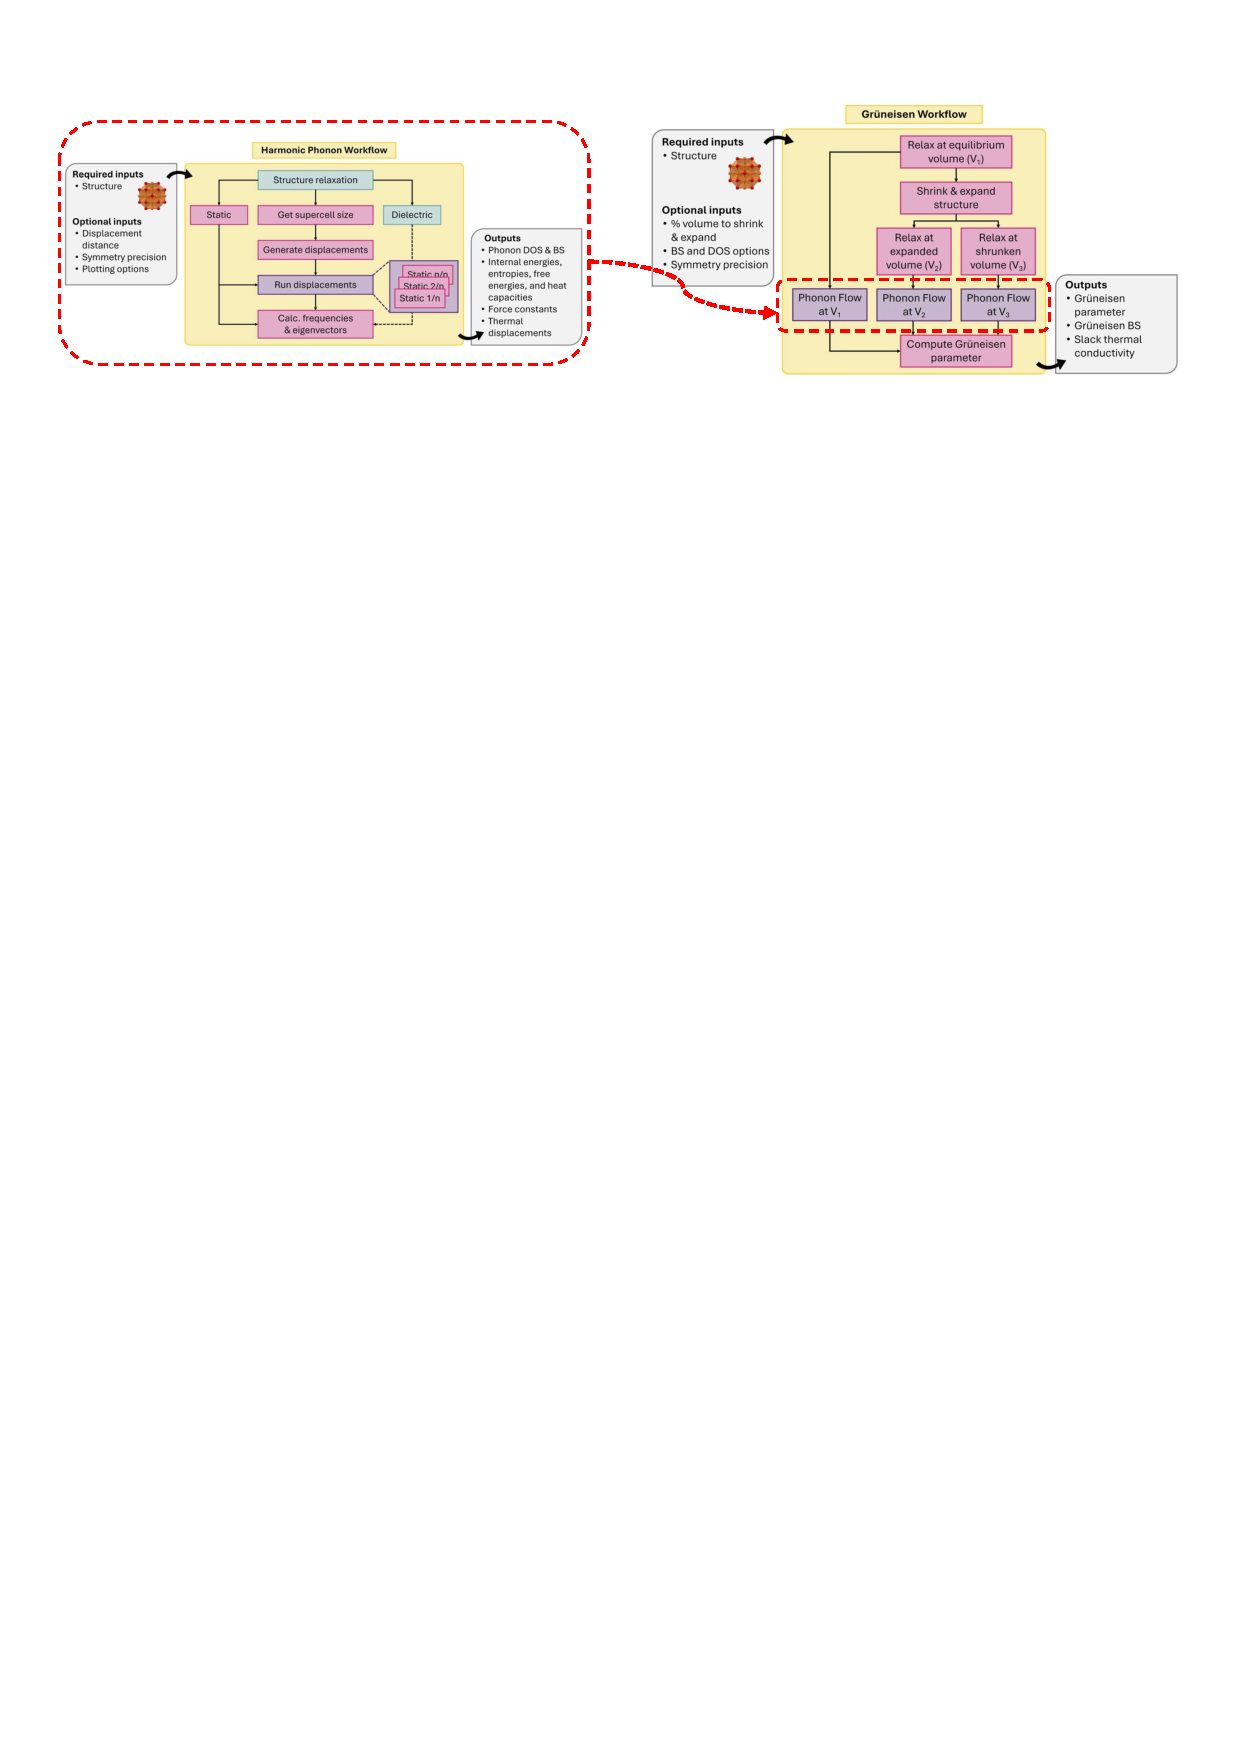
\includegraphics[width=\linewidth]{complex_workflow.pdf}
\caption{Schematic illustrations of the harmonic phonon (left) and the Gr\"{u}neisen parameter (right) calculations workflows as implemented in  Atomate2.\cite{ganose2025atomate2} The composite nature of workflow building in computational materials science is demonstrated by the red dashed error, whereby the more complex Gr\"{u}neisen workflow is built upon the more basic workflow of harmonic phonon calculations.}
    \label{fig:complex_workflow}
\end{figure}


